\section{Experiments}
\label{experiments}
We evaluate our $\mathcal{T}C$-flow and $\mathcal{W}\mathbb{H}C$-flow on three tasks:  structured density estimation, graph reconstruction, and graph generation.\footnote{\url{https://github.com/joeybose/HyperbolicNF}} Throughout our experiments, we rely on three main baselines. %, which are compared against normalizing flows constructed using $\mathcal{T}C$ and $\mathcal{W}\mathbb{H}C$ layers. 
In Euclidean space, we use Gaussian latent variables and affine coupling flows \cite{dinh2016density}, denoted $\mathcal{N}$ and $\mathcal{N}C$, respectively. In the Lorentz model, we use Wrapped Normal latent variables, $\mathbb{H}$-VAE, as an analogous baseline \cite{nagano2019wrapped}. Since all model parameters are defined on tangent spaces, models can be trained with conventional optimizers like Adam \cite{kingma2014adam}. Following previous work, we also consider the curvature $K$ as a learnable parameter with a warmup of $10$ epochs,
and we clamp the max norm of vectors to $40$ before any logarithmic or exponential map \cite{skopek2019mixed}. Appendix E contains details on model architectures and implementation details. 

\subsection{Structured Density Estimation}
We first consider structured density estimation in a canonical VAE setting \cite{kingma2013auto}, where we seek to learn rich approximate posteriors using normalizing flows and evaluate the marginal log-likelihood of test data. Following work on hyperbolic VAEs, we test the approaches on a branching diffusion process (BDP) and dynamically binarized MNIST \cite{mathieu2019continuous,skopek2019mixed}. 

To estimate the log likelihood we perform importance sampling using 500 samples from the test set \cite{burda2015importance}. Our results are shown in Tables \ref{table:bdp_table} and \ref{table:mnist_table}.
On both datasets we observe our hyperbolic flows provide improvements when using latent spaces of low dimension.
This result matches theoretical expectations---\eg, that trees can be perfectly embedded in $\mathbb{H}^2_K$---and dovetails with previous work on graph embedding \cite{nickel2017poincare}. This highlights that the benefit of leveraging hyperbolic space is most prominent in small dimensions. However, as we increase the latent dimension, the Euclidean approaches can compensate for this intrinsic geometric limitation. In the case of BDP we note that the data is indeed a noisy binary tree, which theoretically can be represented in a 2-D hyperbolic space and thus moving to higher dimensional latent space is not beneficial.  
\cut{
and we observe significant gains on both datasets when the latent dimension is small.\cut{In particular, $\mathcal{W}\mathbb{H}C$ performs the best with 2-dimensional latents with a relative improvement of \red{\%XX} over $\mathcal{N}C$ normalizing flows.} We reconcile this result by recalling that even in two dimensions hyperbolic spaces have more room to embed hierarchies. As we increase the latent dimension however we see that Euclidean based approaches outperform our proposed models which are line with similar observation in prior work \cite{nickel2017poincare}.}

\begin{table}[ht]
\begin{small}
\begin{center}
\begin{tabular}{lccccr}
    \toprule
    Model   &  BDP-2 & BDP-4 & BDP-6\\
    \midrule
    $\mathcal{N}$-VAE & $-55.4_{\pm 0.2}$  & $-55.2_{\pm 0.3}$& $-56.1_{\pm 0.2}$   \\
    $\mathbb{H}$-VAE & $-\textbf{54.9}_{\pm 0.3}$& $-55.4_{\pm 0.2}$ &  $-58.0_{\pm 0.2}$\\
    \cut{$\mathcal{P}$-VAE$^*$ & $-55.6_{\pm 0.2}$ & - &-  \\}
    \cut{$\mathbb{U}$-VAE & &  & $-55.8_{\pm 0.4}$  \\}
    $\mathcal{N}C$ & $-55.4_{\pm 0.4}$ & $ \textbf{-54.7}_{\pm 0.1}$ & $\textbf{-55.2}_{\pm 0.3}$  \\
    $\mathcal{T}C$& $\textbf{-54.9}_{\pm 0.1}$& $-55.4_{\pm 0.1}$& $-57.5_{\pm0.2}$\\
    $\mathcal{W}\mathbb{H}C$& $\textbf{-55.1}_{\pm 0.4}$ & $-55.2_{\pm 0.2}$& $-56.9_{\pm 0.4}$\\
    \bottomrule
\end{tabular}
\caption{Test Log Likelihood on Binary Diffusion Process versus latent dimension. All normalizing flows use 2-coupling layers.}
\label{table:bdp_table}
\end{center}
\vskip -0.1in
\end{small}
\end{table}

\begin{table}[ht]
\begin{small}
\begin{center}
\begin{tabular}{lcccc}
    \toprule
    Model   &  \shortstack{MNIST\\2} & \shortstack{MNIST\\4} & \shortstack{MNIST\\6}  \\
    \midrule
    $\mathcal{N}$-VAE &$-139.5_{\pm 1.0}$& $-115.6_{\pm0.2}$ & $-100.0_{\pm0.02}$ \\
    $\mathbb{H}$-VAE & $*$ & $-113.7_{\pm0.9}$& $-99.8_{\pm0.2}$ \\
    \cut{$\mathcal{P}$-VAE$^*$ & $-142.5_{\pm 0.4}$ & $-97.7_{\pm0.2}$&  \\}
    \cut{$\mathbb{U}$-VAE$^*$ & - & $-97.3_{\pm 0.2}$ &  \\}
    $\mathcal{N}C$ &  $-139.2_{\pm 0.4}$ & $-115.2_{\pm0.6}$& $\textbf{-98.7}_{0.3}$ \\
    $\mathcal{T}C$  & $*$& $ \textbf{-112.5}_{\pm0.2}$&$-99.3_{\pm0.2}$  \\
    $\mathcal{W}\mathbb{H}C$ & $\textbf{-136.5}_{\pm 2.1}$ & $\textbf{-112.8}_{\pm0.5}$ &$-99.4_{\pm0.2}$ \\
    \bottomrule
\end{tabular}
\caption{Test Log Likelihood on MNIST averaged over 5 runs verus latent dimension. * indicates numerically unstable settings.}
\label{table:mnist_table}
\end{center}
\vskip -0.1in
\vspace{-13pt}
\end{small}
\end{table}

\subsection{Graph Reconstruction}
We evaluate the practical utility of our hyperbolic flows by conducting experiments on the task of link prediction using graph neural networks (GNNs) \cite{scarselli2008graph} as an inference model. Given a simple graph $\mathcal{G}=(\V,A, X)$, defined by a set of nodes $\mathcal{V}$, an adjacency matrix $A \in \mathbb{Z}^{|\mathcal{V}| \times |\mathcal{V}|}$ and node feature matrix $X \in \mathbb{R}^{|\mathcal{V}| \times n}$, we learn a VGAE \cite{kipf2016variational} model whose inference network, $q_\phi$, defines a distribution over node embeddings $q_\phi(Z | A, X)$. To score the likelihood of an edge existing between pairs of nodes we use an inner product decoder: $p(A_{u,v}=1|z_u,z_v) = \sigma(z_u^Tz_v)$ (with dot products computed in $\mathcal{T}_{\textbf{o}}\mathbb{H}^n_K$ when necessary). Given these components, the inference GNNs are trained to maximize the variational lower bound on a training set of edges. 

We use two different disease datasets taken from \citep{chami2019hyperbolic} and \citep{mathieu2019continuous}\footnote{We uncovered issues with the two remaining datasets in \cite{mathieu2019continuous} and thus omit them (Appendix \ref{dataset_issues}).} for evaluation purposes. Our chosen datasets reflect important real world use cases where the data is known to contain hierarchies. One such measure to determine how tree-like a given graph is known to be Gromov’s $\delta$-hyperbolicity and traditional link prediction datasets such as Cora and Pubmed \cite{yang2016revisiting} were found to lack such a property and are not suitable candidates to evaluate our proposed approach \cite{chami2019hyperbolic}. The first dataset Diseases-\RNum{1} is composed of a network of disorders and disease genes linked by the known disorder–gene associations \cite{goh2007human}. In the second dataset Diseases-\RNum{2}, we build tree networks of a SIR disease spreading model \cite{anderson1992infectious}, where node features determine the susceptibility to the disease. In Table \ref{graph_embeddings_table} we report the AUC and average precision (AP) on the test set.
We observe consistent improvements when using hyperbolic $\mathcal{W}\mathbb{H}C$ flow. Similar to the structured density estimation setting, the performance gains of $\mathcal{W}\mathbb{H}C$ are best observed in low-dimensional latent spaces.

\begin{table}[ht]
\begin{small}
\begin{center}
\begin{tabular}{lcccc}
    \toprule
    Model   & \shortstack{Dis-\RNum{1}\\AUC} & \shortstack{Dis-\RNum{1}\\AP}  & \shortstack{Dis-\RNum{2}\\AUC} & \shortstack{Dis-\RNum{2}\\AP}  \\
    \midrule
    $\mathcal{N}$-VAE & $0.90_{\pm 0.01}$ &
    $0.92_{\pm 0.01}$ &
    $0.92_{\pm 0.01}$ &
    $0.91_{\pm 0.01}$
    
    \\
    $\mathbb{H}$-VAE & $0.91_{\pm 5\textnormal{e-3}}$ &
    $0.92_{\pm 5\textnormal{e-3}}$ &
    $0.92_{\pm 4\textnormal{e-3}}$ &
    $0.91_{\pm 0.01}$ 
    
    \\
    $\mathcal{N}C$ & $0.92_{\pm 0.01}$ &
    $0.93_{\pm 0.01}$ &
     $0.95_{\pm 4\textnormal{e-3}}$ &
    $0.93_{\pm 0.01}$ 
    
    \\
    $\mathcal{T}C$ & $\textbf{0.93}_{\pm 0.01}$ &
    $0.93_{\pm 0.01}$ &
   $\textbf{0.96}_{\pm 0.01}$ &
     $0.95_{\pm 0.01}$ 
    
    \\
    $\mathcal{W}\mathbb{H}C$ & $\textbf{0.93}_{\pm 0.01}$&
    $\textbf{0.94}_{\pm 0.01}$ &
    $\textbf{0.96}_{\pm 0.01}$ &
    $\textbf{0.96}_{\pm 0.01}$
    \\
    \bottomrule
\end{tabular}
\end{center}
\end{small}
\caption{Test AUC and Test AP on Graph Embeddings where Dis-\RNum{1} has latent dimesion 6 and Dis-\RNum{2} has latent dimension 2.}
\label{graph_embeddings_table}
\vskip -0.1in
\end{table}

\subsection{Graph Generation}

Finally, we explore the utility of our hyperbolic flows for generating hierarchical structures. 
As a synthetic testbed, we construct datasets containing uniformly random trees as well as uniformly random lobster graphs \cite{golomb1996polyominoes}, where each graph contains between 20 to 100 nodes. Unlike prior work on graph generation ---i.e. \cite{liu2019graph}, our datasets are designed to have explicit hierarchies and thus enabling us to test the utility of hyperbolic generative models.
We then train a generative model to learn the distribution of these graphs. 
We expect the hyperbolic flows to provide a significant benefit for generating valid random trees, as well as learning the distribution of lobster graphs, which are a special subset of trees. 

We follow the two-stage training procedure outlined in Graph Normalizing Flows \cite{liu2019graph} in that we first train an autoencoder to give node-level latents on which we train an NF for density estimation. Empirically, we find that using GRevNets \cite{liu2019graph} and defining edge probabilities using a distance-based decoder consistently leads to better generation performance. Thus we define edge probabilities as $p(A_{u,v}=1|z_u,z_v) = \sigma((-d_{\mathcal{G}}(u,v) - b)/\tau)$ where $b$ and $\tau$ are learned edge specific bias and temperature parameters. At inference time, we first sample the number of nodes to generate from the empirical distribution of the dataset. We then independently sample node latents from our prior, beginning with a fully connected graph, and then push these samples through our learned flow to give refined edge probabilities. 

\begin{figure*}
    \centering
    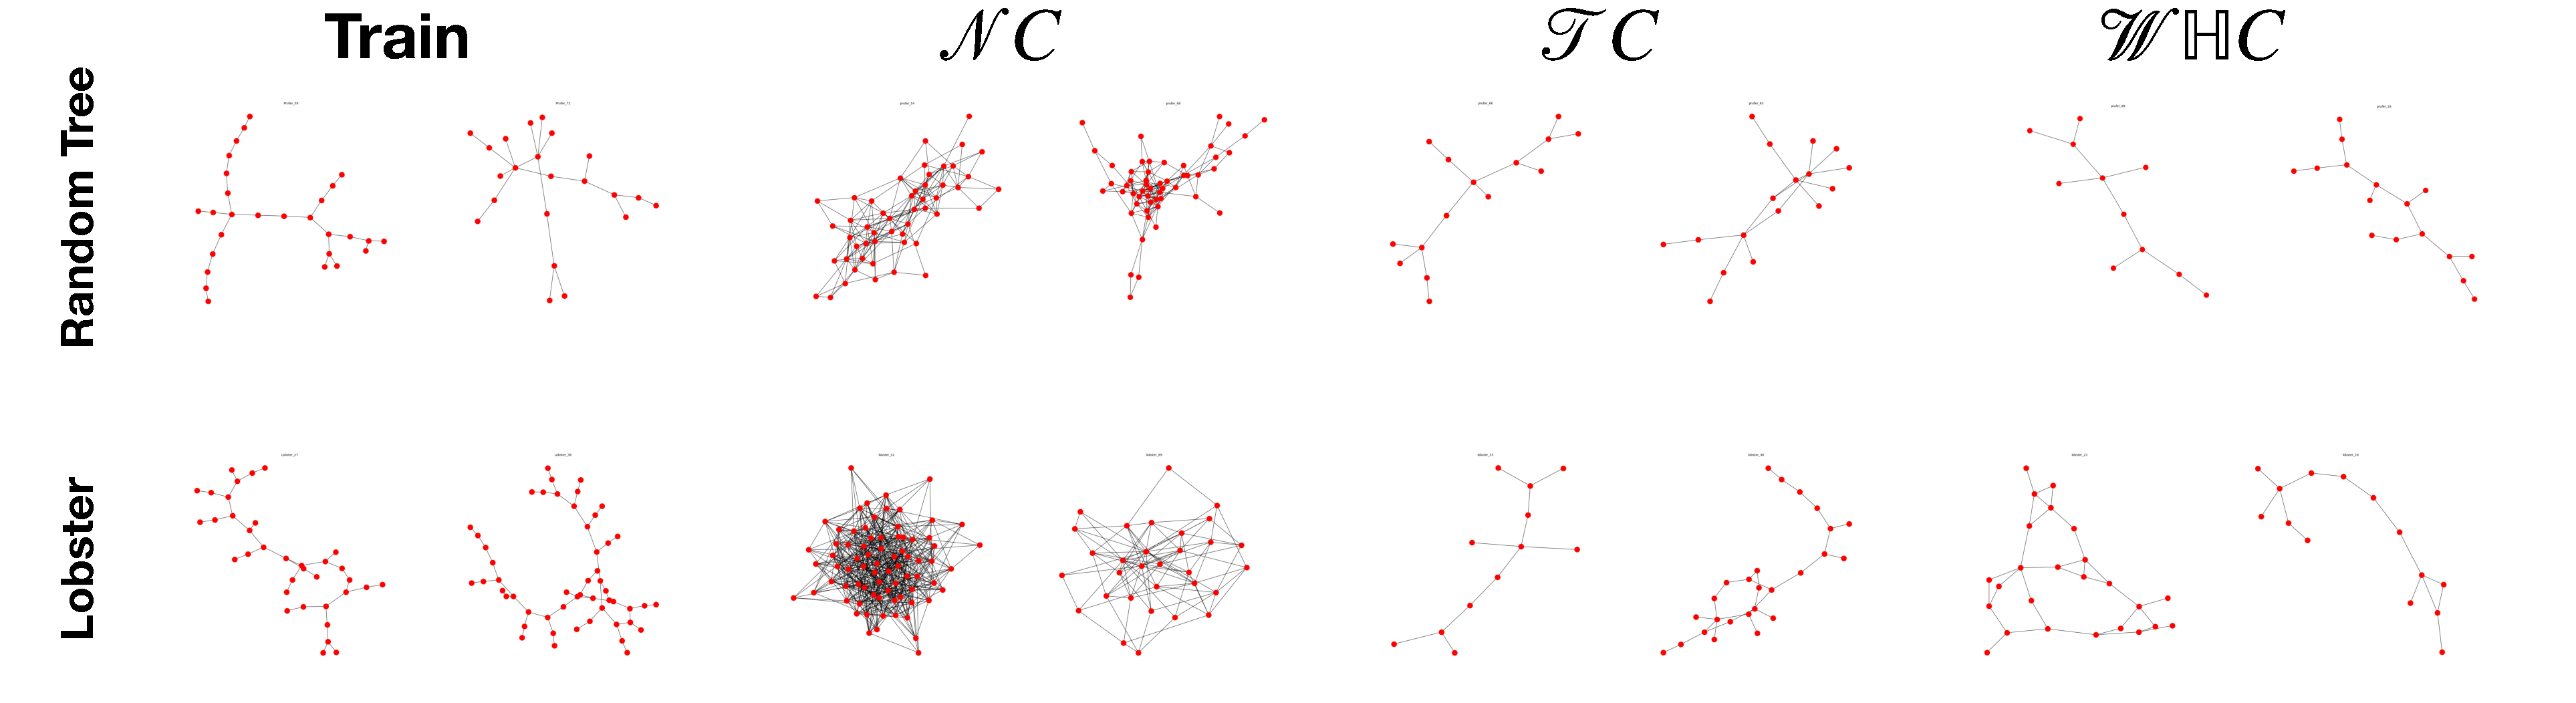
\includegraphics[width=\textwidth]{hyperbolic_graph_gen.pdf}
    \vspace{-5mm}
    \caption{Selected qualitative results on graph generation for lobster and random tree graph.}
    \label{fig:graph_generation_pic}
\end{figure*}

To evaluate the various approaches, we construct $100$ training graphs for each dataset to train our model.
Figure \ref{fig:graph_generation_pic} shows representative samples generated by the various approaches.
We see that hyperbolic normalizing flows learn to generate tree-like graphs and also match the specific properties of the lobster graph distribution, whereas the Euclidean flow model tends to generate densely connected graphs with many cycles (or else disconnected graphs). 
To quantify these intuitions, Table \ref{tab:randtrees} contains statistics on how often the different models generate valid trees (denoted by ``accuracy''), as well as the average number of triangles and the average global clustering coefficients for the generated graphs. 
Since the target data is random trees, a perfect model would achieve 100\% accuracy, with no triangles, and a global clustering of 0 for all graphs. As a representative Euclidean baseline we employ Graph Normalizing Flows (GNFs) which is denoted as $\mathcal{N}C$ in Table \ref{tab:randtrees} and Figure \ref{fig:lobster_graph_gen}.
We see that the hyperbolic models generate valid trees more often, and they generate graphs with fewer triangles and lower clustering on average.
Finally, to evaluate how well the models match the specific properties of the lobster graphs, we follow \citet{liao2019efficient} and report the MMD distance between the generated graphs and a test set for various graph statistics (Figure \ref{fig:lobster_graph_gen}).
Again, we see that the hyperbolic approaches significantly outperform the Euclidean normalizing flow. 

\begin{table}[]
\label{graph_gen_table}
\begin{center}
\begin{tabular}{llll}
    \toprule
    Model   & Accuracy & Avg. Clust. & Avg. GC.\\
    \midrule
    $\mathcal{N}C$ & $56.6_{\pm 5.5}$ & $40.9_{\pm 42.7}$ & $0.34_{\pm0.10}$\\
    $\mathcal{T}C$ & $32.1_{\pm 1.9}$ & $98.3_{\pm 89.5}$ & $0.25_{\pm 0.12}$\\
    $\mathcal{W}\mathbb{H}C$ & $\textbf{62.1}_{\pm 10.9}$ & $\textbf{21.1}_{\pm 13.4}$ & $\textbf{0.13}_{\pm0.07}$\\
    \bottomrule
\end{tabular}
\end{center}
\caption{Generation statistics on random trees over $5$ runs.}
\label{tab:randtrees}
\vspace{-15pt}
\end{table}

\begin{figure}
    \centering
    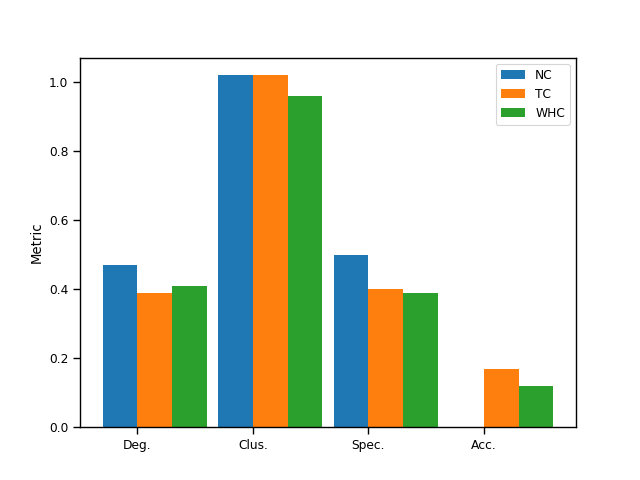
\includegraphics[width=0.85\linewidth]{lobster_graph_gen.png}
    \vspace{-15pt}
    \caption{MMD scores for graph generation on Lobster graphs. Note, that $\mathcal{N}C$ achieves $0\%$ accuracy.}
    \label{fig:lobster_graph_gen}
    \vspace{-15pt}
\end{figure}

